\chapter{MD StepEdit Page:}

The MD StepEdit page is used to program MCL's internal sequencer for a selected track. The programmed sequence will run alongside the MD's sequence for the same track.

\screenshot{step.png}

\textit{To enter the MD StepEdit Page: First select desired track on the MD \textbf{[Function + Track N]}. Then press \textbf{[PageSelect + Trigger 5]}.}

%\fbox{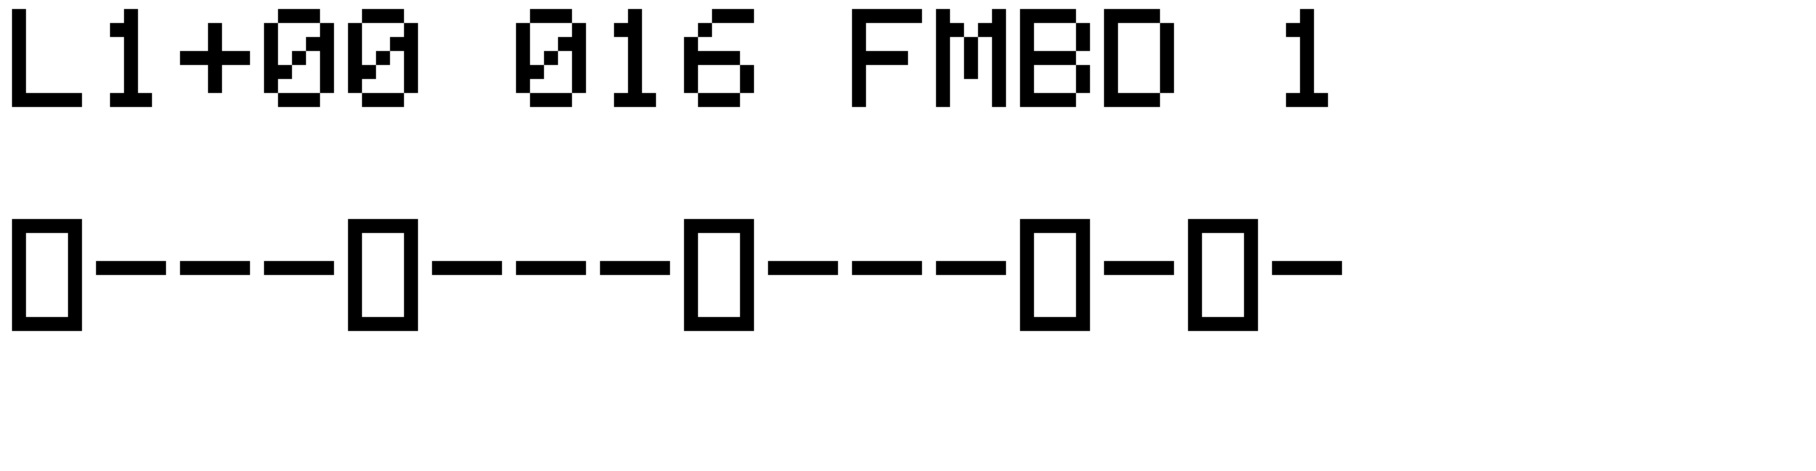
\includegraphics[scale=.40]{seq_step_page.png}}
\screenshot{step_action.png}

\encodersbuttons{Trig Condition}{Micro-Timing}{Track Length}{Note}{Toggles MD/Ext}{PageSelect}{Rotate View}{Track/Trig Menu}

\section{GUI:}
\begin{itemize}
\item The Step Edit Page uses the TI. The trigger buttons on the MD correspond to the 16 steps on the current page of the current track.
\item The 16 steps are displayed on the bottom row
\item Trig Conditions and Micro-Timing settings are per step and are chosen from encoders 1 and 2 respectively.
\end{itemize}

\section{Trig Conditions:}
\begin{itemize}
\item L1,L2,L3,L4,L5,L6,L7,L8 (For Ln, step is only triggered after every n iterations of track)
\item P10, P25, P50, P75, P90 (For Pxx, step has a xx percent chance of being triggered)
\item 1S. (One Shot trig, step is only triggered once)
\end{itemize}

\vspace{-0.3cm}

\section{Program a sequence:}
\begin{itemize}
\item Press and hold trigger button(s) on the MD to place triggers in the sequence.
\item Rotate encoders 1 and 2 to change the conditional mode or micro-timing if desired.
\end{itemize}

\vspace{-0.3cm}

\section{Clearing a sequence:}
\begin{itemize}
\item To clear the current track, press and hold the\textbf{ [ Shift2 ]} to open the track menu, rotate \textbf{[Encoder2]} to the entry \textbf{CLEAR}, then rotate \textbf{[Encoder1]} to select \textbf{TRK}.
\item To clear all MD tracks, select \textbf{ALL}
\end{itemize}

\vspace{-0.3cm}

\section{Rotating visible sequence:}
Each track consists of 4 pages of 16 steps, for a total of 64 steps per track.
\begin{itemize}
\item Rotate the current track-page by pressing the \textbf{[Write] }button.
\end{itemize}

\vspace{-0.3cm}

\section{Changing track length:}
\begin{itemize}
\item Track length is controlled by rotating \textbf{[ Encoder 3 ]}. Only steps less than the current track length are drawn.
\item To change the lengths of all 16 tracks simultaneously hold down \textbf{[Write]} whilst rotating \textbf{[ Encoder 3 ]}.
\item Track length can also be set by holding \textbf{[Write]} and then selecting the corresponding step from the MD trigger interface. The track length is offset by the current track-page.
\end{itemize}

\vspace{-0.3cm}

\section{Chromatic Step Edit:}

\vspace{-0.3cm}

%\fbox{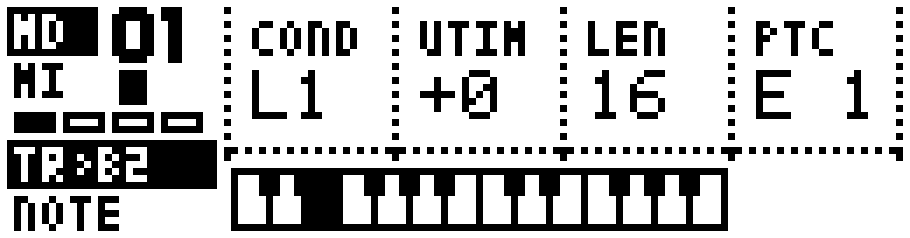
\includegraphics[scale=.40]{step_keyboard.png}}
\screenshot{step_keyboard.png}

The step page allows you to adjust a step's pitch by setting a note value. 
\begin{itemize}
\item Press and hold trigger button(s) on the MD. Rotating \textbf{[ Encoder 4 ]} will allow you change the note value of the selected steps.
\item A keyboard will be drawn on the display, showing the current note.
\end{itemize}
